

\section{Vektorgeometrie}

\begin{definition}{Vektor}
    Objekt, das Betrag und Richtung hat.
    \begin{itemize}
        \item $\overrightarrow{0} = $ Nullvektor (Betrag = 0, einziger Vektor ohne Richtung)
        \item $\overrightarrow{e} = $ Einheitsvektor (Betrag = 1), evtl. mit Index $\vec{e_a}$
        \item $\vec{PQ}=$ Vektor, der den Punkt $P$ in $Q$ verschiebt
        \item $\vec{a} = \vec{b} \Leftrightarrow \abs{\vec{a}} = \abs{\vec{b}}$ und $\vec{a} \parallel \vec{b}$ (selber Betrag und Richtung)
    \end{itemize}
    Es wird zwischen \textit{Orts-} und \textit{Richtungsvektoren} unterschieden.
\end{definition}

\begin{minipage}{0.6\linewidth}
    \begin{definition}{Gegenvektor}
        $-\vec{a}$ ist parallel zu $\vec{a}$, hat denselben Betrag,
        aber entgegengesetzte Richtung. 
    \end{definition}
    \end{minipage}
    \begin{minipage}{0.25\linewidth}
        {\small
        $$-\overrightarrow{a} = \begin{pmatrix}
            -a_x \\
            -a_y
            \end{pmatrix}$$}
    \end{minipage}
    \begin{minipage}{0.13\linewidth}
        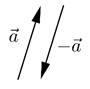
\includegraphics[width=0.8\linewidth]{vec-gegen.png}
    \end{minipage}

\begin{definition}{Länge/Betrag eines Vektors}
    $\abs{\vec{a}}=\sqrt{a_1^2+a_2^2+\cdots+a_n^2}$
\end{definition}

\begin{formula}{Einheitsvektor/Normierung}
    {\large
    $\vec{e_a}=\frac{1}{a}\cdot\vec{a} \quad = \quad \frac{\overrightarrow{a}}{|\overrightarrow{a}|}$}

    Der Vektor $\vec{e_a}$ wird als \textbf{Einheitsvektor oder auch normiert} bezeichnet 
    und der Übergang von $\vec{a}$ nach $\vec{e_a}$ heisst \textbf{Normierung}.
\end{formula}



\begin{definition}{Orthogonal (Senkrecht)} $\overrightarrow{a} \cdot \overrightarrow{b} = 0 \rightarrow \text{ orthogonal}$

    $\vec{a}$ und $\vec{b}$ sind orthogonal, wenn der Winkel zwischen ihnen 90° beträgt
\end{definition}

\begin{definition}{Normalenvektor}
    Ein Normalenvektor, der orthogonal zu einer Ebene $E$ ist, heisst \textit{Normalenvektor} von $E$.
    Eine Koordinatendarstellung einer Ebene $E$ heisst normiert, wenn gilt: $\vec{n}=1$.
\end{definition}



\raggedcolumns

\paragraph*{Rechnen mit Vektoren}

\begin{minipage}{0.5\linewidth}
    \begin{formula}{Vektoraddition}\\
        $\overrightarrow{a} + \overrightarrow{b} = \begin{pmatrix} a_x + b_x\\ a_y + b_y \end{pmatrix}$
    \end{formula}
\end{minipage}
\begin{minipage}{0.5\linewidth}
\begin{formula}{Skalarmultiplikation}\\
    $\lambda \cdot \overrightarrow{a} = \begin{pmatrix}
    \lambda \cdot a_x \\
    \lambda \cdot a_y
    \end{pmatrix}$
\end{formula}
\end{minipage}

\raggedcolumns

\begin{formula}{Skalarprodukt} 
    $\overrightarrow{a} \cdot \overrightarrow{b} = a_x \cdot b_x + a_y \cdot b_y = |\overrightarrow{a}| \cdot |\overrightarrow{b}| \cdot \cos(\varphi)$
\end{formula}

\begin{formula}{Winkelberechnung} {\small $\varphi$ = Winkel zwischen $\vec{a}$ und $\vec{b}$ ($0\le\phi\le\pi$)}
    $$\cos(\varphi) = \frac{\overrightarrow{a} \cdot \overrightarrow{b}}{|\overrightarrow{a}| \cdot |\overrightarrow{b}|} = \frac{a_x b_x + a_y b_y}{\sqrt{a_x^2 + a_y^2} \cdot \sqrt{b_x^2 + b_y^2}  } $$
\end{formula}


\begin{minipage}{0.55\linewidth}
\begin{concept}{Winkel und Skalarprodukt}\\
    Seien $\vec{a}$ und $\vec{b}$ zwei Vektoren und $\varphi$ der eingeschlossene Winkel, 
    $0\leq\varphi\leq\pi$, dann gilt:
\end{concept}
\end{minipage}
\begin{minipage}{0.35\linewidth}
    $\varphi<\frac{\pi}{2},\, \text{ wenn } \vec{a}\cdot\vec{b} > 0 \\  
    \varphi>\frac{\pi}{2},\, \text{ wenn } \vec{a}\cdot\vec{b} < 0 \\   
    \varphi=\frac{\pi}{2},\, \text{ wenn } \vec{a}\cdot\vec{b} = 0 $
\end{minipage}

\begin{theorem}{Eigenschaften des Skalarprodukts}\\ Für beliebige Vektoren $\vec{a}$, $\vec{b}$, $\vec{c}$ und Skalaren $\lambda\in\R$ gilt:
    \begin{itemize}
        \item $\vec{a}\cdot\vec{a}=\abs{\vec{a}}^2$
        \item $(-\lambda)\cdot\vec{a}=-(\lambda\cdot\vec{a})=\lambda\cdot(-\vec{a})$
        \item Kommutativ-Gesetz: $\vec{a}\cdot\vec{b}=\vec{b}\cdot\vec{a}$
        \item Distributiv-Gesetze: $\vec{a}\cdot(\vec{b}+\vec{c})=\vec{a}\cdot\vec{b}+\vec{a}\cdot\vec{c}$ und $(\vec{a}+\vec{a})\cdot\vec{c}=\vec{a}\cdot\vec{c}+\vec{b}\cdot\vec{c}$
        \item Gemischtes Assoziativ-Gesetz: $\lambda\cdot(\vec{a}\cdot\vec{b})=(\lambda\cdot\vec{a})\cdot\vec{b}=\vec{a}\cdot(\lambda\cdot\vec{b})$
    \end{itemize} 
\end{theorem}

\begin{minipage}{0.8\linewidth}
\begin{formula}{Kreuzprodukt} {\small $\overrightarrow{a} \times \overrightarrow{b}$ ist orthogonal zu $\overrightarrow{a}$ und $\overrightarrow{b}$
        $$\overrightarrow{a} \times \overrightarrow{b} = \left(\begin{array}{ccc}
            a_y \cdot b_z &-& a_z \cdot b_y \\
            a_z \cdot b_x &-& a_x \cdot b_z \\
            a_x \cdot b_y &-& a_y \cdot b_x
            \end{array}\right)$$
    \vspace{2mm}
    $|\overrightarrow{a} \times \overrightarrow{b}| = |\overrightarrow{a}| \cdot |\overrightarrow{b}| \cdot \sin(\varphi) 
        \quad \quad \quad \overrightarrow{a} \times \overrightarrow{b} \neq \overrightarrow{b} \times \overrightarrow{a}$
    
        \vspace{1mm}

        Für $\R^2$ gilt: $\overrightarrow{a} \times \overrightarrow{b} = a_x \cdot b_y - a_y \cdot b_x$
        }
\end{formula}
\end{minipage}
\begin{minipage}{0.19\linewidth}
    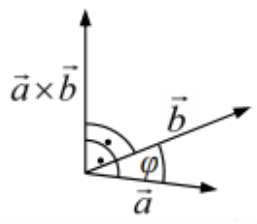
\includegraphics[width=1\linewidth]{vektorprodukt.png}
\end{minipage}  

\begin{theorem}{Eigenschaften des Kreuzprodukts} auch genannt Vektorprodukt\\
    Für beliebige Vektoren $\vec{a}$, $\vec{b}$, $\vec{c}$ und Skalaren $\lambda\in\R$ gilt:
    \begin{itemize}
        \item $\vec{a}\times\vec{a}=\vec{0}$
        \item Antikommutativ-Gesetz: $\vec{a}\times\vec{b}=-(\vec{b}\times\vec{a})$
        \item Distributiv-Gesetz: $\vec{a}\times(\vec{b}+\vec{c})=\vec{a}\times\vec{b}+\vec{a}\times\vec{c}$
        \item Gemischtes Assoziativ-Gesetz:
            $\lambda\cdot(\vec{a}\times\vec{b})=(\lambda\cdot\vec{a})\times\vec{b}=\vec{a}\times(\lambda\cdot\vec{b})$ 
    \end{itemize}
    \textcolor{pink}{$\vec{a}\times(\vec{b}\times\vec{c})\ne(\vec{a}\times\vec{b})\times\vec{c}$!!}
\end{theorem}

\begin{formula}{Fläche des aufgespannten Parallelogramms} = $\vec{a}\times\vec{b}$\\
    \begin{minipage}{0.6\linewidth}
    $$h = |\overrightarrow{b}| \cdot \sin(\varphi)$$
    $$A = |\overrightarrow{a}| \cdot h = |\overrightarrow{a} \times \overrightarrow{b}| = |\overrightarrow{a}| \cdot |\overrightarrow{b}| \cdot \sin(\varphi)$$
    \end{minipage}
    \hspace{3mm}
    \begin{minipage}{0.35\linewidth}
        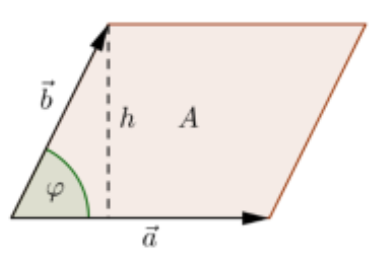
\includegraphics[width=0.7\linewidth]{parallelogramm.png}
    \end{minipage}
\end{formula}



\begin{minipage}{0.7\linewidth}
    \begin{formula}{Orthogonal Projektion}von $\overrightarrow{b}$ auf $\overrightarrow{a}$
            $$\vec{b}_a=\frac{\vec{a}\cdot\vec{b}}{\abs{\vec{a}}^2}\cdot\vec{a}   
            \text{ und }
            \abs{\vec{b}}_a=\frac{\abs{\vec{a}\cdot\vec{b}}}{\abs{\vec{a}}}  $$
    \end{formula}
\end{minipage}
    \begin{minipage}{0.25\linewidth}
        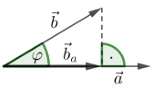
\includegraphics[width=0.9\linewidth]{vec-proj.png}
    \end{minipage}
    \begin{remark}
        Die erste Formel gilt für $0<\varphi\leq\frac{\pi}{2}$,
        die zweite für $\frac{\pi}{2}<\varphi\leq\pi$
    \end{remark}


\paragraph*{Lineare Abhängigkeit und Komponentendarstellung}

\begin{definition}{Linearkombination (LK)}
    $\lambda_1\cdot\vec{a_1}+\lambda_2\cdot\vec{a_2}+\ldots+\lambda_n\cdot\vec{a_n}$
    
    \vspace*{2mm}

    mit $\lambda_n\in R$ heisst \textit{Linearkombination} der Vektoren $\vec{a_1},\ldots,\vec{a_n}$.
\end{definition}

\begin{definition}{Lineare Abhängigkeit}
    $\overrightarrow{a_{1}}, \overrightarrow{a_{2}}, \ldots, \overrightarrow{a_{k}}$ sind linear unabhängig, wenn:
    \vspace*{1mm}
    \begin{itemize}
    \item $\lambda_{1} \cdot \overrightarrow{a_{1}}+\lambda_{2} \cdot \overrightarrow{a_{2}}+\cdots+\lambda_{k} \cdot \overrightarrow{a_{k}} \neq \overrightarrow{0}(\lambda>0 \wedge \lambda \in \mathbb{R})$
    \item $0 \cdot \overrightarrow{a_{1}}+0 \cdot \overrightarrow{a_{2}}+\cdots+0 \cdot \overrightarrow{a_{k}}$ als einzige LK $\overrightarrow{0}$ ergibt
\end{itemize}
\end{definition}

\begin{definition}{Komponentendarstellung} $\vec{a}=a_1\cdot\vec{e}_1+\cdots+a_n\cdot\vec{e}_n=
    \begin{psmallmatrix}
        a_1\\\scalebox{0.5}{\vdots}\\a_n
    \end{psmallmatrix}$

    $\exists a_1, ... a_n \in \R$ (Komponente), so dass
    jeder Vektor $\vec{a}$ \\als LK von $\vec{e}_1,...\vec{e}_n$
    eindeutig dargestellt werden kann. 
\end{definition}

\begin{definition}{Ortsvektor}
    $\vec{r}(P)=\overrightarrow{OP}=x_1\cdot\vec{e}_1+...+x_n\cdot\vec{e}_n =
    \begin{psmallmatrix}
        x_1\\\scalebox{0.5}{\vdots}\\x_n
    \end{psmallmatrix}$
    
    Zu jedem Punkt $P$ des Vektorraums definiert! Ortsvektoren sind im Ursprung $O$ angeheftet, wie jeder Vektor LK 
    von $\vec{e_1}, ... \vec{e_n}$ und lassen sich in Komponentenschreibweise darstellen:
\end{definition}

\begin{minipage}{0.6\linewidth}
\begin{formula}{Komponentendarstellung von $\overrightarrow{OP}$}
    
    $\vec{r}(Q)=\vec{r}(P)+\overrightarrow{PQ}\\
    \Rightarrow \overrightarrow{PQ}=\vec{r}(Q)-\vec{r}(P)=\begin{pmatrix}
        x_Q-x_P\\
        y_Q-y_P\\
        \cdots-\cdots
    \end{pmatrix}$
\end{formula}
\end{minipage}
\begin{minipage}{0.38\linewidth}
    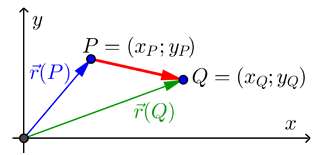
\includegraphics[width=\linewidth]{vec-komp-calc.png}
\end{minipage}


\raggedcolumns


\subsubsection*{Geraden und Ebenen}

\paragraph*{Kollinear und Komplanar}   

\begin{definition}{Kollinear} $\vec{a}$ und $\vec{b}$\\
    \begin{minipage}{0.8\linewidth}
    \begin{itemize}
        \item $\exists$ eine Gerade $g$, zu der beide parallel sind
        \item Spezialfall: Nullvektor ist zu jedem Vektor kollinear
        \item $\vec{a} \times \vec{b} = \vec{0}$ (Kreuzprodukt)
        \item $\vec{a}=\lambda\cdot\vec{b}$ (einer ist Vielfaches des anderen)
    \end{itemize}
    \end{minipage}
    \hspace{3mm}
    \begin{minipage}{0.1\linewidth}
        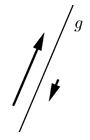
\includegraphics[width=1\linewidth]{vec-kollinear.png}
    \end{minipage}
\end{definition}

\begin{theorem}{Lage} von Geraden im Raum\\
    \vspace*{2mm}
    %make a table to show the different cases
    \begin{tabular}{c|c|c|}
        & Gemeinsame Punkte & keine gem. Punkte \\
        \hline
        Kollinear & Identisch & echt Parallel \\
        \hline
        nicht kollinear & Schneidend & Windschief \\
        \hline
    \end{tabular}
\end{theorem}

\begin{minipage}{0.8\linewidth}
\begin{definition}{Komplanar} $\vec{a}$, $\vec{b}$ und $\vec{c}$\\
    Es existiert eine Ebene $E$, zu der alle parallel sind.
\end{definition}
\end{minipage}
\begin{minipage}{0.15\linewidth}
    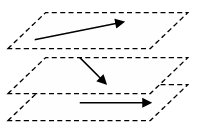
\includegraphics[width=\linewidth]{vec-komplanar.png}
\end{minipage}

\begin{minipage}{0.7\linewidth}
    \begin{theorem}{LK komplanarer Vektoren} $\vec{a}$, $\vec{b}$ und $\vec{c}$\\
        Wenn $\vec{a}$ und $\vec{b}$ nicht kollinear sind lässt sich $\vec{c}$ als Linearkombination von $\vec{a}$ und $\vec{b}$ mit $\lambda, \mu \in \R$ darstellen:
            {\large$\vec{c}=\lambda\cdot\vec{a}+\mu\cdot\vec{b}$}
    \end{theorem}
    \end{minipage}
    \begin{minipage}{0.25\linewidth}
        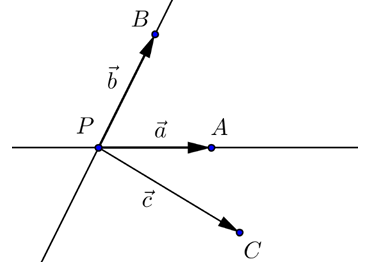
\includegraphics[width=\linewidth]{vec-kompl.png}
\end{minipage}

\begin{minipage}{0.7\linewidth}
    \begin{theorem}{LK nicht komplanarer Vektoren} $\vec{a}$, $\vec{b}$ und $\vec{c}$\\
        Jeder Vektor $\vec{d}$ im $\R^3$ lässt sich als Linearkombination von $\vec{a}$, $\vec{b}$ und $\vec{c}$ eindeutig darstellen:
            {\large$\vec{d}=\lambda\cdot\vec{a}+\mu\cdot\vec{b}+\nu\cdot\vec{c}$}
    \end{theorem}
    \end{minipage}
    \begin{minipage}{0.25\linewidth}
        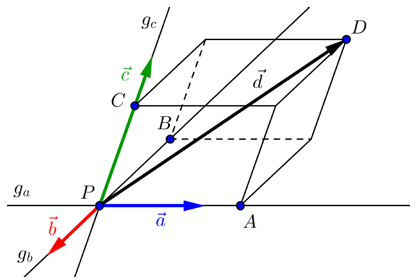
\includegraphics[width=\linewidth]{vec-nicht-kompl.png}
\end{minipage}

\paragraph{Darstellungsformen von Ebenen und Geraden}

\begin{minipage}{0.6\linewidth}
    \begin{definition}{Parameterdarstellung} einer Geraden
        $$\overrightarrow{r}(A) = \overrightarrow{r}(P) + \lambda \cdot \overrightarrow{PQ}$$
    
        {\small Der Punkt $P$ heisst \textit{Aufpunkt}, der Vektor $\overrightarrow{a} = \overrightarrow{PQ}$ heisst \textit{Richtungsvektor} von $g$.}
    \end{definition}
\end{minipage}
\begin{minipage}{0.4\linewidth}
    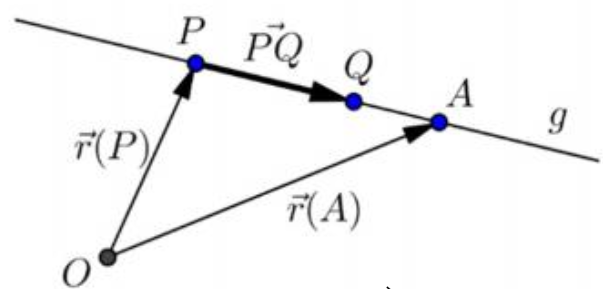
\includegraphics[width=1\linewidth]{gerade.png}\\
    $g: \overrightarrow{r}(P) + \lambda \cdot \overrightarrow{a}$
\end{minipage}


\begin{minipage}{0.6\linewidth}
\begin{definition}{Parameterdarstellung} einer Ebene
    $$E:\,\vec{r}(P)+\lambda\cdot\vec{a}+\mu\cdot\vec{b}\, (\lambda,\mu\in\R)$$
    $P$ = \textit{Aufpunkt}, $a=\overrightarrow{PQ}$ und 
    $\vec{b}=\overrightarrow{PR}$ sind \textit{Richtungsvektoren} von $E$.\\

    Parameterdarstellung nicht eindeutig!\\ Richtungsvektoren zwei beliebige
    Vektoren: \textit{parallel} zu $E$ und \textit{nicht kollinear}
\end{definition}
\end{minipage}
\begin{minipage}{0.4\linewidth}
    \begin{center}
    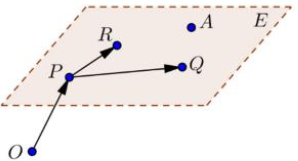
\includegraphics[width=0.8\linewidth]{ebene.png}
    \end{center}
    $\overrightarrow{PA}$, $\overrightarrow{PR}$, $\overrightarrow{PQ}$ komplanar\\

    $\overrightarrow{PA} = \lambda \cdot \overrightarrow{PR} + \mu \cdot \overrightarrow{PQ}$
\end{minipage}


\begin{definition}{Koordinatendarstellung} $a,b,c,d\in \R$
    $$E:\,ax+by+cz+d=0$$
    Bedeutung: die Ebene E besteht aus allen Punkten $P$, deren Koordinaten
    $x, y$ und $z$ diese Gleichung erfüllen.
    $\abs{d}$ = Abstand zum Ursprung, wenn Gleichung normiert
    (sonst $\frac{\vec{d}}{\vec{n}}$)
    {\small
    $$\vec{n} = \begin{pmatrix} a \\ b \\ c \end{pmatrix}, \quad
    \vec{n} \perp \begin{pmatrix} x \\ y \\ z \end{pmatrix}, \quad
    \begin{pmatrix} x \\ y \\ z \end{pmatrix} \cdot \begin{pmatrix} a \\ b \\ c \end{pmatrix} = 0$$
    }
\end{definition}

\paragraph*{Umrechnung von Parameter- und Koordinatendarstellung}

\begin{formula}{Umrechnung Parameterdarstellung zu Koordinatendarstellung}\\
    Berechnen über den Normalenvektor aus dem Kreuzprodukt der Richtungsvektoren,
    welches die Koeffizienten $a, b$ und $c$ liefert. 
    Der Aufpunkt wird über das Einsetzen eines Punktes der Ebene $E$ ermittelt.
    $$
        \vec{n}=\vec{a}\times\vec{b}=\begin{psmallmatrix}
            a\\b\\c
        \end{psmallmatrix}
    $$
\end{formula}

\begin{example2}{Parameterdarstellung $\rightarrow$ Koordinatendarstellung}
    $$E: \begin{psmallmatrix} 2 \\ 4 \\ 1 \end{psmallmatrix} + \lambda \cdot \begin{psmallmatrix} 1 \\ 3 \\ 1 \end{psmallmatrix} + \mu \cdot \begin{psmallmatrix} 2 \\ 2 \\ -4 \end{psmallmatrix}$$
    $$\vec{n} = \begin{psmallmatrix} 1 \\ 3 \\ 1 \end{psmallmatrix} \times \begin{psmallmatrix} 2 \\ 2 \\ -4 \end{psmallmatrix} = \begin{psmallmatrix} -12 -2 \\ 2 + 4 \\ 2 - 6 \end{psmallmatrix} = \begin{psmallmatrix} -14 \\ -6 \\ -4 \end{psmallmatrix}$$
    $$E: -14x - 6y - 4z + d = 0$$
    Aufpunkt einsetzen: $-14 \cdot 2 - 6 \cdot 4 - 4 \cdot 1 + d = 0 \Rightarrow d = 8$
\end{example2}

\begin{formula}{Umrechnung Koordinatendarstellung zu Parameterdarstellung}\\
    Um eine Koordinatendarstellung in eine Parameterdarstellung umzurechnen,
    werden drei Punkte berechnet.
    Einer dieser Punkte wird dann als aufpunkt gewählt und mit den restlichen
    werden Richtungsvektoren berechnet.
\end{formula}

\begin{example2}{Koordinatendarstellung $\rightarrow$ Parameterdarstellung}
    $$E: 2x + 7y - 4z + 1 = 0$$
    Punkte einsetzen: $(0|0|z), (1|0|z), (0|1|z)$\\
    \begin{minipage}{0.5\linewidth}
    \begin{itemize}
        \item $2 \cdot 0 + 7 \cdot 0 - 4 \cdot z + 1 = 0 \Rightarrow z = \frac{1}{4}$
        \item $2 \cdot 1 + 7 \cdot 0 - 4 \cdot z + 1 = 0 \Rightarrow z = \frac{3}{4}$
        \item $2 \cdot 0 + 7 \cdot 1 - 4 \cdot z + 1 = 0 \Rightarrow z = \frac{8}{4}$
    \end{itemize}
    \end{minipage}
    \hspace{2mm}
    \begin{minipage}{0.45\linewidth}
    $E: \begin{psmallmatrix} 0 \\ 0 \\ \frac{1}{4} \end{psmallmatrix} +
    \lambda \begin{psmallmatrix} 1 \\ 0 \\ \frac{2}{4} \end{psmallmatrix} +
    \mu \begin{psmallmatrix} 0 \\ 1 \\ \frac{7}{4} \end{psmallmatrix}$
    \end{minipage}
\end{example2}



\paragraph*{Abstände berechnen}


\begin{formula}{Abstand Punkt-Gerade}Gesucht ist der Fusspunkt $B\in g$\\
    Gegeben: Gerade $g=\vec{r}(P)+\lambda\cdot\vec{a}$ in Parameterform und Punkt $A$
    
    \begin{minipage}{0.59\linewidth}
        \begin{enumerate}
            \item Da $B\in g\Rightarrow \vec{r}(B)=\vec{r}(P)+\lambda_B\cdot\vec{a}$ 
            \item $\vec{BA}=\vec{r}(A)-\vec{r}(B)$
            \item $\vec{BA}\perp g\Rightarrow\vec{BA}\cdot\vec{a}=0$
            \item $l=\abs{\vec{BA}}$ ($\lambda_B$ in $\vec{BA}$ einsetzen)
        \end{enumerate}
    \end{minipage}
    \begin{minipage}{0.4\linewidth}
        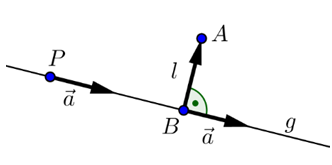
\includegraphics[width=1\linewidth]{vec-abstand-von-punkt.png}
    \end{minipage}

    Meist einfacher:
    $\vec{PA}=\vec{r}(A)-\vec{r}(P) \Rightarrow l=\frac{\abs{\vec{PA}\times\vec{a}}}{\abs{\vec{a}}}$   
\end{formula}

\begin{formula}{Abstand Punkt-Ebene} $l$ = Abstand von $A$ zu $E$\\
    \begin{minipage}{0.7\linewidth}
    Gegeben: Punkt $A=(x_A;y_A;z_A)$, Ebene $E$ mit der \textbf{normierten} 
    Koordinatendarstellung $E:\,ax+by+cz+d=0$
    \begin{center}
    $l=\abs{ax_A+by_A+cz_A+d}$
    \end{center}
    \end{minipage}
    \hspace{3mm}
    \begin{minipage}{0.2\linewidth}
        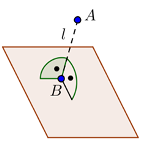
\includegraphics[width=1\linewidth]{vec-abstand-von-ebene.png}
    \end{minipage}

    \begin{minipage}{0.65\linewidth}
        \textbf{nicht normierte} Koordinatendarstellung:
    $$l=\frac{\abs{ax_A+by_A+cz_A+d}}{\abs{\vec{n}}}$$
    \end{minipage}
    \begin{minipage}{0.3\linewidth}
        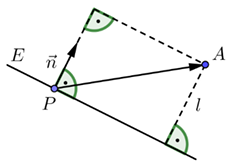
\includegraphics[width=0.9\linewidth]{vec-abstand-von-ebene2.png}
    \end{minipage}
\end{formula}


\section{Geometrische Transformationen}

\subsection{$\R^2$}

\begin{formula}{Streckung}\\
    \begin{minipage}{0.4\linewidth}
        \begin{itemize}
            \item in $x$-Richtung um $\lambda_1$
            \item in $y$-Richtung um $\lambda_2$
        \end{itemize}
    \end{minipage}
    \begin{minipage}{0.6\linewidth}
        $$\begin{pmatrix} x' \\ y' \end{pmatrix} = \begin{pmatrix} \lambda_1 & 0 \\ 0 & \lambda_2 \end{pmatrix} \cdot \begin{pmatrix} x \\ y \end{pmatrix}$$
    \end{minipage}
\end{formula}

\begin{formula}{Spiegelung}\\
    \begin{minipage}{0.45\linewidth}
        \begin{itemize}
            \item Gerade $g: ax + by = 0$
            \item mit $a^2 + b^2 = 1$
        \end{itemize}
    \end{minipage}
    \begin{minipage}{0.5\linewidth}
        $$\begin{pmatrix} 1 - 2a^2 & -2ab \\ -2ab & 1 - 2b^2 \end{pmatrix}$$
    \end{minipage}
\end{formula}

\begin{example}
    \begin{minipage}{0.5\linewidth}
        \begin{itemize}
            \item Gerade $g: x + 7y = 0$
            \item Normiert $g: \frac{1}{\sqrt{50}} x + \frac{7}{\sqrt{50}} y = 0$
        \end{itemize}
    \end{minipage}
    \begin{minipage}{0.45\linewidth}
        $$\frac{1}{50} \cdot \begin{pmatrix} 48 & -14 \\ -14 & -48 \end{pmatrix}$$
    \end{minipage}
\end{example}

\begin{formula}{Orthogonale Projektion}\\
    \begin{minipage}{0.5\linewidth}
    \begin{itemize}
        \item auf Gerade $g: ax + by = 0$
        \item mit $a^2 + b^2 = 1$
    \end{itemize}
    \end{minipage}
    \begin{minipage}{0.5\linewidth}
    $$\begin{pmatrix} 1 - a^2 & -ab \\ -ab & 1-b^2 \end{pmatrix}$$
    \end{minipage}
\end{formula}

\begin{example}
    \begin{minipage}{0.5\linewidth}
    \begin{itemize}
        \item Gerade $g: 2x -y = 0$
        \item Normiert $g: \frac{2}{\sqrt{5}} x - \frac{1}{\sqrt{5}} y = 0$ 
    \end{itemize}
    \end{minipage}
    \begin{minipage}{0.45\linewidth}
    $$\frac{1}{5} \cdot \begin{pmatrix} 1 & 2 \\ 2 & 4 \end{pmatrix}$$
    \end{minipage}
\end{example}

\begin{formula}{Rotation}\\
    \begin{minipage}{0.35\linewidth}
    \begin{itemize}
        \item um den Ursprung
        \item um Winkel $\alpha$
    \end{itemize}
    \end{minipage}
    \begin{minipage}{0.65\linewidth}
    $$\begin{pmatrix} x' \\ y' \end{pmatrix} = \begin{pmatrix} \cos(\alpha) & -\sin(\alpha) \\ \sin(\alpha) & \cos(\alpha) \end{pmatrix} \cdot \begin{pmatrix} x \\ y \end{pmatrix}$$
    \end{minipage}
\end{formula}

\begin{formula}{Scherung}\\
    \begin{minipage}{0.5\linewidth}
    \begin{itemize}
        \item in $x$-Richtung um $s_1$
        \item in $y$-Richtung um $s_2$
    \end{itemize}
    \end{minipage}
    \begin{minipage}{0.5\linewidth}
    $$\begin{pmatrix} x' \\ y' \end{pmatrix} = \begin{pmatrix} 1 & s_1 \\ s_2 & 1 \end{pmatrix} \cdot \begin{pmatrix} x \\ y \end{pmatrix}$$
    \end{minipage}
\end{formula}

\columnbreak

\subsection*{$\R^3$}

\begin{formula}{Zentrische Streckung}\\
    \begin{minipage}{0.4\linewidth}
    \begin{itemize}
        \item in $x$-Richtung um $\lambda_1$
        \item in $y$-Richtung um $\lambda_2$
        \item in $z$-Richtung um $\lambda_3$
    \end{itemize}
    \end{minipage}
    \begin{minipage}{0.5\linewidth}
    $$\begin{pmatrix} x' \\ y' \\ z' \end{pmatrix} = \begin{pmatrix} \lambda_1 & 0 & 0 \\ 0 & \lambda_2 & 0 \\ 0 & 0 & \lambda_3 \end{pmatrix} \cdot \begin{pmatrix} x \\ y \\ z \end{pmatrix}$$
    \end{minipage}
\end{formula}

\begin{formula}{Spiegelung} an der Ebene\\
    \begin{minipage}{0.45\linewidth}
    \begin{itemize}
        \item Ebene $E: ax + by + cz = 0$
        \item mit $a^2 + b^2 + c^2 = 1$
    \end{itemize}
    \end{minipage}
    \begin{minipage}{0.5\linewidth}
    $$\begin{pmatrix} 1 - 2a^2 & -2ab & -2ac \\ -2ab & 1 - 2b^2 & -2bc \\ -2ac & -2bc & 1 - 2c^2 \end{pmatrix}$$
    \end{minipage}
    $$S = E - 2\vec{n} \cdot \vec{n}^T$$
\end{formula}

\begin{example}
    \begin{minipage}{0.5\linewidth}
    \begin{itemize}
        \item Ebene $E: x + 2y + 3z = 0$
        \item Normiert $E: \frac{1}{\sqrt{14}} x + \frac{2}{\sqrt{14}} y + \frac{3}{\sqrt{14}} z = 0$
    \end{itemize}
    \end{minipage}
    \begin{minipage}{0.45\linewidth}
    $$\frac{1}{14} \cdot \begin{pmatrix} 11 & 4 & 6 \\ 4 & 7 & 6 \\ 6 & 6 & 7 \end{pmatrix}$$
    \end{minipage}
\end{example}

\begin{formula}{Orthogonale Projektion} auf die Ebene\\
    \begin{minipage}{0.5\linewidth}
    \begin{itemize}
        \item Ebene $E: ax + by + cz = 0$
        \item mit $a^2 + b^2 + c^2 = 1$
    \end{itemize}
    \end{minipage}
    \begin{minipage}{0.5\linewidth}
    $$\begin{pmatrix} 1 - a^2 & -ab & -ac \\ -ab & 1 - b^2 & -bc \\ -ac & -bc & 1 - c^2 \end{pmatrix}$$
    \end{minipage}
    $$P = E - \vec{n} \cdot \vec{n}^T$$
\end{formula}

\begin{example}
    \begin{minipage}{0.5\linewidth}
    \begin{itemize}
        \item Ebene $E: 2x - y + 3z = 0$
        \item Normiert $E: \frac{2}{\sqrt{14}} x - \frac{1}{\sqrt{14}} y + \frac{3}{\sqrt{14}} z = 0$
    \end{itemize}
    \end{minipage}
    \begin{minipage}{0.45\linewidth}
    $$\frac{1}{14} \cdot \begin{pmatrix} 13 & 4 & 6 \\ 4 & 13 & 9 \\ 6 & 9 & 13 \end{pmatrix}$$
    \end{minipage}
\end{example}

\begin{formula}{Rotation}um den Winkel $\alpha$ um die x, y, z Achsen\\
    \begin{minipage}{0.45\linewidth}
    $$\text{x: } \begin{pmatrix} 1 & 0 & 0 \\ 0 & \cos(\alpha) & -\sin(\alpha) \\ 0 & \sin(\alpha) & \cos(\alpha) \end{pmatrix}$$
    \end{minipage}
    \begin{minipage}{0.45\linewidth}
    $$\text{y: } \begin{pmatrix} \cos(\alpha) & 0 & \sin(\alpha) \\ 0 & 1 & 0 \\ -\sin(\alpha) & 0 & \cos(\alpha) \end{pmatrix}$$
    \end{minipage}
    \\
    $$\text{z: } \begin{pmatrix} \cos(\alpha) & -\sin(\alpha) & 0 \\ \sin(\alpha) & \cos(\alpha) & 0 \\ 0 & 0 & 1 \end{pmatrix}$$
    
\end{formula}


\begin{formula}{Rotation} um den Winkel $\alpha$ um die Gerade g
    
    Gerade $g: \vec{r} = \vec{a} + t \cdot \vec{b}$ mit $|\vec{b}| = 1$

    $\vec{a}$ ist ein Punkt auf der Geraden g, $\vec{b}$ ist der Richtungsvektor der Geraden g

    \vspace{3mm}
   
    $\begin{pmatrix} \cos(\alpha) + a^2(1 - \cos(\alpha)) & ab(1 - \cos(\alpha)) - b \sin(\alpha) & ... \\ 
        ab(1 - \cos(\alpha)) + b \sin(\alpha) & \cos(\alpha) + b^2(1 - \cos(\alpha)) & ... \\ 
        -a \sin(\alpha) + b(1 - \cos(\alpha)) & b \sin(\alpha) + a(1 - \cos(\alpha)) & ... \end{pmatrix}$  
    
    \begin{flushright}
    $\begin{pmatrix} ... & ... & a \sin(\alpha) + b(1 - \cos(\alpha)) \\ 
        ... & ... & -b \sin(\alpha) + a(1 - \cos(\alpha)) \\ 
        ... & ... & \cos(\alpha) + (a^2 + b^2)(1 - \cos(\alpha)) \end{pmatrix}$  
    \end{flushright}

        \vspace{3mm}

        {\small $\uparrow$ 3x3 Matrix, die die Rotation um die Gerade g beschreibt (hat nicht auf eine Zeile gepasst)}
\end{formula}



\section*{LGS und Matrizen}

\subsubsection*{Matrizen}

    \begin{definition}{Matrix}
        Tabelle mit $m$ Zeilen und $n$ Spalten: $m \times n$-Matrix $A$\\
        $a_{ij}$: Element in der $i$-ten Zeile und $j$-ten Spalte
    \end{definition}
    
    \begin{minipage}{0.5\linewidth}
    \begin{formula}{Addition und Subtraktion}
        \begin{itemize}
            \item $A + B = C$
            \item $c_{ij} = a_{ij} + b_{ij}$
        \end{itemize}
    \end{formula}
    \end{minipage}
    \begin{minipage}{0.5\linewidth}
    \begin{formula}{Skalarmultiplikation}
        \begin{itemize}
            \item $k \cdot A = B$
            \item $b_{ij} = k \cdot a_{ij}$
        \end{itemize}
    \end{formula}
    \end{minipage}

    \begin{theorem}{Rechenregeln für die Addition und skalare Multiplikation von Matrizen}
        Kommutativ-, Assoziativ- und Distributiv-Gesetz gelten für Matrix-Addition
    \end{theorem}
    
    \begin{formula}{Matrixmultiplikation} $A^{m \times n}$, $B^{n \times k}$\\
        \begin{minipage}{0.6\linewidth}
        Bedingung: $A$ $n$ Spalten, $B$ $n$ Zeilen.\\
        Resultat: $C$ hat $m$ Zeilen und $k$ Spalten.
        \begin{itemize}
            \item $A \cdot B = C$
            \item $c_{ij} = a_{i1} \cdot b_{1j} + a_{i2} \cdot b_{2j} + \ldots + a_{in} \cdot b_{nj}$
            \item $A \cdot B \neq B \cdot A$
        \end{itemize}  
        \end{minipage}
        \begin{minipage}{0.35\linewidth} 
        \begin{center}
        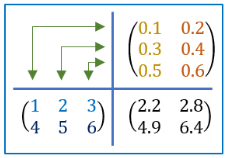
\includegraphics[width=0.8\linewidth]{matrixmultiplikation.png}
        \end{center}
        \end{minipage}
    \end{formula}
    
     \begin{theorem}{Rechenregeln für die Multiplikation von Matrizen}\\
        Assoziativ, Distributiv, nicht Kommutativ!
    \end{theorem}

    \begin{minipage}{0.65\linewidth}
        \begin{definition}{Transponierte Matrix} $A^{m \times n} \rightarrow (A^T)^{n \times m}$
            \begin{itemize}
                \item $A^T$: Spalten und Zeilen vertauscht
                \item $(A^T)_{ij} = A_{ji}$ und ${(A\cdot B)}^T = B^T\cdot A^T$
            \end{itemize}
        \end{definition}
    \end{minipage}
    \begin{minipage}{0.35\linewidth}
        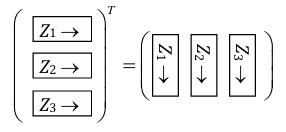
\includegraphics[width=1\linewidth]{mat-transpos.png}
    \end{minipage}

    \begin{KR}{Spezielle Matrizen}
        \begin{itemize}
            \item \textbf{Symmetrische Matrix}: $A^T = A$
            \item \textbf{Einheitsmatrix}: $E$ mit $e_{ij} = 1$ für $i = j$ und $e_{ij} = 0$ für $i \neq j$
            \item \textbf{Diagonalmatrix}: $a_{ij} = 0$ für $i \neq j$
            \item \textbf{Dreiecksmatrix}: $a_{ij} = 0$ für $i > j$ (obere Dreiecksmatrix) \\oder $i < j$ (untere Dreiecksmatrix)
        \end{itemize}
    \end{KR}

\subsubsection*{Lineare Gleichungssysteme (LGS)}
    
        \begin{definition}{Lineares Gleichungssystem (LGS)}
            Ein \textit{lineares Gleichungssystem} ist eine Sammlung von Gleichungen, 
            die linear in den Unbekannten sind. 
            Ein LGS kann in Matrixform $A\cdot\vec{x}=\vec{b}$ dargestellt werden.\\
            \begin{minipage}
                {0.45\linewidth}
                {\small
                $A$: Koeffizientenmatrix\\
                $\vec{x}$: Vektor der Unbekannten\\
                $\vec{b}$: Vektor der Konstanten}
            \end{minipage}
            \begin{minipage}{0.55\linewidth}
                $\begin{psmallmatrix} a_{11} & \cdots & a_{1n} \\ \scalebox{0.5}{\vdots} & \cdots & \scalebox{0.5}{\vdots} \\ a_{m1} & \cdots & a_{mn} \end{psmallmatrix} \cdot \begin{psmallmatrix}
                    x_1 \\ \scalebox{0.5}{\vdots} \\ x_n
                \end{psmallmatrix} = \begin{psmallmatrix}
                    b_1 \\ \scalebox{0.5}{\vdots} \\ b_m
                \end{psmallmatrix}$
            \end{minipage}
        \end{definition}

    
        \begin{theorem}{Rang einer Matrix} $rg(A)$ = Anzahl Zeilen - Anzahl Nullzeilen
            
            $\Rightarrow$ Anzahl linear unabhängiger Zeilen- oder Spaltenvektoren
        \end{theorem}


\begin{concept}{Zeilenstufenform (Gauss)}
    \begin{itemize}
        \item Alle Nullen stehen unterhalb der Diagonalen, Nullzeilen zuunterst
        \item Die erste Zahl $\neq 0$ in jeder Zeile ist eine führende Eins
        \item Führende Einsen, die weiter unten stehen $\rightarrow$ stehen weiter rechts
    \end{itemize}
    \textbf{Reduzierte Zeilenstufenform: (Gauss-Jordan)}\\
    Alle Zahlen links und rechts der führenden Einsen sind Nullen.
\end{concept}

\begin{KR}{Zeilenperationen} erlaubt bei LGS (z.B. Gauss-Verfahren)
        \begin{itemize}
            \item Vertauschen von Zeilen
            \item Multiplikation einer Zeile mit einem Skalar
            \item Addition eines Vielfachen einer Zeile zu einer anderen
        \end{itemize}
    \end{KR}
    
    \begin{formula}{Gauss-Jordan-Verfahren}
        \begin{enumerate}
            \item bestimme linkeste Spalte mit Elementen $\neq 0$ (Pivot-Spalte)
            \item oberste Zahl in Pivot-Spalte $= 0$\\ $\rightarrow$ vertausche Zeilen so dass $a_{11} \neq 0$
            \item teile erste Zeile durch $a_{11}$ $\rightarrow$ so erhalten wir führende Eins
            \item Nullen unterhalb führender Eins erzeugen (Zeilenperationen)
        \end{enumerate}
        nächste Schritte: ohne bereits bearbeitete Zeilen Schritte 1-4 wiederholen, bis Matrix Zeilenstufenform hat
    \end{formula}

    

    \begin{theorem}{Lösbarkeit von linearen Gleichungssystemen}

        \begin{minipage}{0.5\linewidth}
            \begin{itemize}
                \item Lösbar: $rg(A) = rg(A|b)$
                \item genau eine Lösung: $rg(A) = n$
            \end{itemize}
        \end{minipage}
        \begin{minipage}{0.5\linewidth}
            \begin{itemize}
                \item unendlich viele Lösungen:\\ $rg(A) < n$
            \end{itemize}
        \end{minipage}
    \end{theorem}

    \begin{KR}{Parameterdarstellung} bei unendlich vielen Lösungen

        \begin{minipage}{0.74\linewidth}
            Führende Unbekannte: Spalte mit führender Eins\\
            Freie Unbekannte: Spalten ohne führende Eins
        \end{minipage}
        \begin{minipage}{0.25\linewidth}
            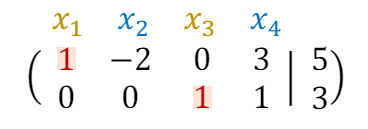
\includegraphics[width=1\linewidth]{parameterdarstellung_lgs.png}
        \end{minipage}

        \vspace{1mm}
        
        Auflösung nach der führenden Unbekannten:
        \begin{itemize}
            \item $1 x_1 - 2 x_2 + 0 x_3 + 3 x_4 = 5 \quad x_2 = \lambda \rightarrow x_1 = 5 + 2 \cdot \lambda - 3 \cdot \mu$
            \item $0 x_1 + 0 x_2 + 1 x_3 + 1 x_4 = 3 \quad x_4 = \mu \rightarrow x_3 = 3 - \mu$    
        \end{itemize}
        \vspace*{2mm}
        $$ \vec{x} = \begin{psmallmatrix} x_1 \\ x_2 \\ x_3 \\ x_4 \end{psmallmatrix} 
        = \begin{psmallmatrix} 5 + 2 \lambda - 3 \mu \\ \lambda \\ 3 - \mu \\ \mu \end{psmallmatrix} 
        = \begin{psmallmatrix} 5 \\ 0 \\ 3 \\ 0 \end{psmallmatrix} + \lambda \begin{psmallmatrix} 2 \\ 1 \\ 0 \\ 0 \end{psmallmatrix} + \mu \begin{psmallmatrix} -3 \\ 0 \\ -1 \\ 1 \end{psmallmatrix}$$
    \end{KR}

    \begin{definition}{Homogenes LGS}
        $\vec{b}=\vec{0} \rightarrow A\cdot\vec{x}=\vec{0} \rightarrow rg(A)=rg(A\mid\vec{b})$\\
        nur zwei Möglichkeiten:
            \begin{itemize}
                \item eine Lösung $x_1=x_2=\cdots=x_n=0$, die sog. \textit{triviale Lösung}.
                \item unendlich viele Lösungen
            \end{itemize}
    \end{definition}

    \begin{theorem}{Koeffizientenmatrix{,} Determinante{,} Lösbarkeit des LGS }\\
        Für $n\times n$-Matrix $A$ sind folgende Aussagen äquivalent:
    
        \vspace{1mm}
    
        \begin{minipage}{0.3\linewidth}
            \begin{itemize}
                \item $\det(A)\neq 0$
                \item $rg(A)=n$
                \item $A$ ist invertierbar
            \end{itemize}
        \end{minipage}
        \begin{minipage}{0.7\linewidth}
            \begin{itemize}
                \item Spalten von $A$ sind linear unabhängig.
                \item Zeilen von $A$ sind linear unabhängig.
                \item LGS $A\cdot\vec{x}=\vec{0}$ \\hat eindeutige Lösung $x=A^{-1}\cdot 0=0$
            \end{itemize}
        \end{minipage}
    \end{theorem}


  

\subsubsection*{Quadratische Matrizen}

\paragraph{Inverse}
    \begin{definition}{Inverse einer quadratischen Matrix A} $A^{-1}$ 
        
        $A^{-1}$ existiert, wenn $rg(A) = n$. $A^{-1}$ ist eindeutig bestimmt.

        \vspace{1mm}

        {\small Eine Matrix heisst \textit{invertierbar / regulär}, wenn sie eine Inverse hat. 
        Andernfalls heisst sie \textit{singulär}}
    \end{definition}
  
    \begin{theorem}{Eigenschaften invertierbarer Matrizen}
        \begin{itemize}
            \item $A\cdot A^{-1}=A^{-1}\cdot A=E$ und $(A^{-1})^{-1}=A$
            \item ${(A\cdot B)}^{-1}=B^{-1}\cdot A^{-1}$ {\small $\quad$ Die Reihenfolge ist relevant!}
            \item $A$ und $B$ invertierbar $\Rightarrow$ $AB$ invertierbar
            \item ${(A^T)^{-1}}={(A^{-1})}^T$ $\quad$ $A$ invertierbar $\Rightarrow$ $A^T$ invertierbar
        \end{itemize}
    \end{theorem}

\begin{theorem}{Inverse einer $2 \times 2$-Matrix} $A = \begin{psmallmatrix} a & b \\ c & d \end{psmallmatrix}$ mit $det(A) = ad - bc$
        $$A^{-1} = \frac{1}{\det(A)} \cdot \begin{pmatrix} d & -b \\ -c & a \end{pmatrix}$$
        NUR Invertierbar falls $ad - bc \neq 0$
\end{theorem}

\begin{KR}{Inverse berechnen} einer quadratischen Matrix $A^{n \times n}$
    $$A \cdot A^{-1} = E \rightarrow \left( A | E \right) \leadsto \text{Zeilenoperationen} \leadsto \left( E | A^{-1}\right)$$
\end{KR}

\begin{concept}{LGS mit Inverse lösen}
    $A \cdot \vec{x} = \vec{b}$
    $$A^{-1} \cdot A \cdot \vec{x} = A^{-1} \cdot \vec{b} \rightarrow \vec{x} = A^{-1} \cdot \vec{b}$$
    Beispiel:\\
    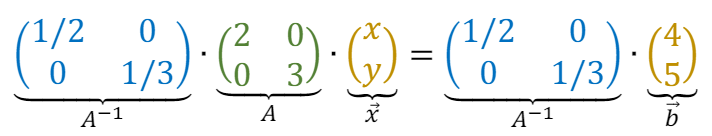
\includegraphics[width=0.7\linewidth]{lgs_inverse.png}
\end{concept}

\subsubsection{Pivotisierung}

\begin{concept}{Permutationsmatrix} $P$ ist eine Matrix, die aus der Einheitsmatrix durch Zeilenvertauschungen entsteht. 
    \vspace{1mm}\\
    \begin{minipage}[t]{0.5\textwidth}
        Für die Vertauschung der $i$-ten und $j$-ten Zeile hat $P_k$ die \textbf{Form}:
        \begin{itemize}
            \item $p_{ii} = p_{jj} = 0$ 
            \item $p_{ij} = p_{ji} = 1$
            \item Sonst gleich wie in $E_n$
        \end{itemize}
    \end{minipage}
    \hspace{3mm}
    \begin{minipage}[t]{0.45\textwidth}
        \vspace{1mm}
        \textbf{Wichtige Eigenschaften}:
        \begin{itemize}
            \item $P^{-1} = P^T = P$
            \item Mehrere Vertauschungen:\\ $P = P_l \cdot ... \cdot P_1$
        \end{itemize}
    \end{minipage}
\end{concept}

\begin{example2}{Zeilenvertauschung} für Matrix A mit Permutationsmatrix $P_1$:
    \vspace{1mm}\\
\begin{minipage}[t]{0.5\textwidth}
    $\underbrace{\begin{psmallmatrix}
    1 & 2 & 3\\
    4 & 5 & 6\\
    7 & 8 & 9
    \end{psmallmatrix}}_{A} \cdot 
    \underbrace{\begin{psmallmatrix}
    0 & 0 & 1\\
    0 & 1 & 0\\
    1 & 0 & 0
    \end{psmallmatrix}}_{P_1} =
    \begin{psmallmatrix}
    7 & 8 & 9\\
    4 & 5 & 6\\
    1 & 2 & 3
    \end{psmallmatrix}$
\end{minipage}
\begin{minipage}[t]{0.45\textwidth}
    \vspace{-2mm}
    $\Rightarrow A \cdot P_1$ bewirkt die Vertauschung von Zeile 1 und 3
\end{minipage}
\end{example2}

\vspace{-1mm}
\subsubsection{Pivotisierung}

\begin{concept}{Spaltenpivotisierung}\\
Strategie zur numerischen Stabilisierung des Gauss-Algorithmus durch Auswahl des betragsmäßig größten Elements als Pivotelement.

Vor jedem Eliminationsschritt in Spalte $i$:
\begin{itemize}
    \item Suche $k$ mit $|a_{ki}| = \max\{|a_{ji}| \mid j = i,\ldots,n\}$
    \item Falls $a_{ki} \neq 0$: Vertausche Zeilen $i$ und $k$
    \item Falls $a_{ki} = 0$: Matrix ist singulär
\end{itemize}
\end{concept}

\begin{KR}{Gauss-Algorithmus mit Pivotisierung}\\
\textbf{1. Elimination (Vorwärts)}:
\begin{itemize}
    \item Für $i=1,\ldots,n-1$:
    \begin{itemize}
    \item Finde $k \geq i$ mit $|a_{ki}| = \max\{|a_{ji}| \mid j = i,\ldots,n\}$
    \item Falls $a_{ki} = 0$: Stop (Matrix singulär)
    \item Vertausche Zeilen $i$ und $k$
    \item Für $j=i+1,\ldots,n$:
    \begin{itemize}
    \item $z_j := z_j - \frac{a_{ji}}{a_{ii}}z_i$
    \end{itemize}
    \end{itemize}
\end{itemize}
\vspace{-2mm}
\resizebox{\columnwidth}{!}{
\textbf{2. Rückwärtseinsetzen}:
$x_i = \frac{b_i - \sum_{j=i+1}^n a_{ij}x_j}{a_{ii}}, \quad i=n,n-1,\ldots,1$
}
\end{KR}

\begin{concept}{Vorteile der Permutationsmatrix}
    \begin{itemize}
        \item Exakte Nachverfolgung aller Zeilenvertauschungen
        \item Einfache Rückführung auf ursprüngliche Reihenfolge durch $P^{-1}$
        \item Kompakte Darstellung mehrerer Vertauschungen
        \item Numerisch stabile Implementierung der Pivotisierung
    \end{itemize}
\end{concept}





\section{Numerische Lösung linearer Gleichungssysteme}

\subsection{Matrix-Zerlegungen}

\begin{definition}{Dreieckszerlegung}
Eine Matrix $A \in \mathbb{R}^{n\times n}$ kann zerlegt werden in:
\vspace{1mm}\\
\begin{minipage}[t]{0.5\textwidth}
    \textbf{Untere Dreiecksmatrix L:}\\
    $l_{ij} = 0$ für $j > i$\\
    Diagonale normiert ($l_{ii}=1$)
\end{minipage}
\hspace{3mm}
\begin{minipage}[t]{0.45\textwidth}
    \textbf{Obere Dreiecksmatrix R:}\\
    $r_{ij} = 0$ für $i > j$\\
    Diagonalelemente $\neq 0$
\end{minipage}
\end{definition}


\subsubsection{LR-Zerlegung}

\begin{theorem}{LR-Zerlegung}\\
Jede reguläre Matrix $A$, für die der Gauss-Algorithmus ohne Zeilenvertauschungen durchführbar ist, lässt sich zerlegen in:
$A = LR$
wobei $L$ eine normierte untere und $R$ eine obere Dreiecksmatrix ist.
\end{theorem}

\begin{KR}{LR-Zerlegung durchführen}
    $(E | A | E) \underbrace{\leadsto}_{Gauss} (P | R | L)$
    \vspace{-3mm}\\
\begin{enumerate}
    \item Zerlegung bestimmen:
    \begin{itemize}
        \item Gauss-Elimination durchführen
        \item Eliminationsfaktoren $-\frac{a_{ji}}{a_{ii}}$ in $L$ speichern
        \item Resultierende obere Dreiecksmatrix ist $R$
    \end{itemize}
    
    \item System lösen:
    \begin{itemize}
        \item Vorwärtseinsetzen: $Ly = b$
        \item Rückwärtseinsetzen: $Rx = y$
    \end{itemize}
    
    \item Bei Pivotisierung:
    \begin{itemize}
        \item Permutationsmatrix $P$ erstellen
        \item $PA = LR$ speichern
        \item $Ly = Pb$ lösen
    \end{itemize}
\end{enumerate}
\end{KR}

\begin{remark}
    $E$ = Einheitsmatrix, $P$ = Permutationsmatrix
\end{remark}


\begin{example2}{LR-Zerlegung}
$\underbrace{\begin{psmallmatrix}
-1 & 1 & 1\\
1 & -3 & -2\\
5 & 1 & 4
\end{psmallmatrix}}_{A}, \underbrace{\begin{psmallmatrix}
0\\
5\\
3
\end{psmallmatrix}}_{b}
\rightarrow \begin{vsmallmatrix}
0 & 0 & 1\\
0 & 1 & 0\\
1 & 0 & 0
\end{vsmallmatrix} \begin{vsmallmatrix}
-1 & 1 & 1\\
1 & -3 & -2\\
5 & 1 & 4
\end{vsmallmatrix}
\begin{vsmallmatrix}
1 & 0 & 0\\
0 & 1 & 0\\
0 & 0 & 1
\end{vsmallmatrix}$

\paragraph{Schritt 1: Erste Spalte}
Max. Element in 1. Spalte: $|a_{31}| = 5$, also Z1 und Z3 tauschen:

\begin{minipage}{0.5\textwidth}
$$\begin{vsmallmatrix}
0 & 0 & 1\\
0 & 1 & 0\\
1 & 0 & 0
\end{vsmallmatrix} \begin{vsmallmatrix}
5 & 1 & 4\\
1 & -3 & -2\\
-1 & 1 & 1
\end{vsmallmatrix}
\begin{vsmallmatrix}
1 & 0 & 0\\
0 & 1 & 0\\
0 & 0 & 1
\end{vsmallmatrix}$$
\end{minipage}
\begin{minipage}{0.45\textwidth}
    \vspace{2mm}
    Eliminationsfaktoren:\\
    $l_{21} = \frac{1}{5}, \quad l_{31} = -\frac{1}{5}$
\end{minipage}


Nach Elimination:
$\begin{vsmallmatrix}
0 & 0 & 1\\
0 & 1 & 0\\
1 & 0 & 0
\end{vsmallmatrix} \begin{vsmallmatrix}
5 & 1 & 4\\
0 & -3.2 & -2.8\\
0 & 1.2 & 1.8
\end{vsmallmatrix}
\begin{vsmallmatrix}
1 & 0 & 0\\
\frac{1}{5} & 1 & 0\\
-\frac{1}{5} & 0 & 1
\end{vsmallmatrix}$

\paragraph{Schritt 2: Zweite Spalte}
Max. Element in 2. Spalte unter Diagonale: $|-3.2| > |1.2|$, \\ keine Vertauschung nötig.
Eliminationsfaktor:
$l_{32} = \frac{1.2}{-3.2} = -\frac{3}{8}$
\vspace{2mm}\\
Nach Elimination:
$\underbrace{\begin{vsmallmatrix}
0 & 0 & 1\\
0 & 1 & 0\\
1 & 0 & 0
\end{vsmallmatrix}}_{P} \underbrace{\begin{vsmallmatrix}
5 & 1 & 4\\
0 & -3.2 & -2.8\\
0 & 0 & 0.75
\end{vsmallmatrix}}_{R}
\underbrace{\begin{vsmallmatrix}
1 & 0 & 0\\
\frac{1}{5} & 1 & 0\\
-\frac{1}{5} & -\frac{3}{8} & 1
\end{vsmallmatrix}}_{L}$

\paragraph{Lösung des Systems}
\begin{enumerate}
    \item $Pb = \begin{psmallmatrix} 3\\ 5\\ 0 \end{psmallmatrix}$
    \item Löse $Ly = Pb$ durch Vorwärtseinsetzen:
    $y = \begin{psmallmatrix} 3\\ 4.4\\ 2.25 \end{psmallmatrix}$
    \item Löse $Rx = y$ durch Rückwärtseinsetzen:
    $x = \begin{psmallmatrix} -1\\ -4\\ 3 \end{psmallmatrix}$
\end{enumerate}

Probe:
$Ax = \begin{psmallmatrix}
-1 & 1 & 1\\
1 & -3 & -2\\
5 & 1 & 4
\end{psmallmatrix} \begin{psmallmatrix} -1\\ -4\\ 3 \end{psmallmatrix} = \begin{psmallmatrix} 0\\ 5\\ 3 \end{psmallmatrix} = b$
\end{example2}

\columnbreak

\subsubsection{QR-Zerlegung}

\begin{concept}{QR-Zerlegung}\\
Eine orthogonale Matrix $Q \in \mathbb{R}^{n\times n}$ erfüllt: $Q^T Q = QQ^T = I_n$
\vspace{1mm}\\
Die QR-Zerlegung einer Matrix $A$ ist: $A = QR$
\vspace{1mm}\\
wobei $Q$ orthogonal und $R$ eine obere Dreiecksmatrix ist.
\end{concept}

\begin{definition}{Householder-Transformation}\\
Eine Householder-Matrix hat die Form:
$H = I_n - 2uu^T$

mit $u \in \mathbb{R}^n$, $\|u\| = 1$. Es gilt:
\begin{itemize}
    \item $H$ ist orthogonal ($H^T = H^{-1}$) und symmetrisch ($H^T = H$)
    \item $H^2 = I_n$
\end{itemize}
\end{definition}

\begin{KR}{QR-Zerlegung mit Householder}
\begin{enumerate}
    \item Initialisierung: $R := A$, $Q := I_n$
    \item Für $i = 1,\ldots,n-1$:
        \begin{itemize}
            \item Bilde Vektor $v_i$ aus i-ter Spalte von $R$ ab Position $i$
            \item $w_i := v_i + \text{sign}(v_{i1})\|v_i\|e_1$
            \item $u_i := w_i/\|w_i\|$
            \item $H_i := I_{n-i+1} - 2u_iu_i^T$
            \item Erweitere $H_i$ zu $Q_i$ durch $I_{i-1}$ links oben
            \item $R := Q_iR$ und $Q := QQ_i^T$
        \end{itemize}
\end{enumerate}
\end{KR}

\begin{example2}[breakable]{QR-Zerlegung mit Householder}
    %TODO: check if this is correct and/or relevant - either correct or replace with better example
$A = \begin{psmallmatrix}
2 & 5 & -1\\
-1 & -4 & 2\\
0 & 2 & 1
\end{psmallmatrix}$

\paragraph{Schritt 1: Erste Spalte}
Erste Spalte $a_1$ und Einheitsvektor $e_1$:
$a_1 = \begin{psmallmatrix} 2\\ -1\\ 0 \end{psmallmatrix}, \quad e_1 = \begin{psmallmatrix} 1\\ 0\\ 0 \end{psmallmatrix}$

Householder-Vektor für erste Spalte:
\vspace{1mm}
\begin{enumerate}
    \item Berechne Norm: $|a_1| = \sqrt{2^2 + (-1)^2 + 0^2} = \sqrt{5}$
    \vspace{1mm}
    \item Bestimme Vorzeichen: $\text{sign}(a_{11}) = \text{sign}(2) = 1$
         \begin{itemize}
              \item Wähle positives Vorzeichen, da erstes Element positiv
              \item Dies maximiert die erste Komponente von $v_1$
              \item Verhindert Auslöschung bei der Subtraktion
         \end{itemize}
         \vspace{1mm}
    \item $v_1 = a_1 + \text{sign}(a_{11})|a_1|e_1 = \begin{psmallmatrix} 2\\ -1\\ 0 \end{psmallmatrix} + \sqrt{5}\begin{psmallmatrix} 1\\ 0\\ 0 \end{psmallmatrix} = \begin{psmallmatrix} 2 + \sqrt{5}\\ -1\\ 0 \end{psmallmatrix}$
    \vspace{1mm}
    \item Normiere $v_1$: $|v_1| = \sqrt{(2 + \sqrt{5})^2 + 1} \Rightarrow
            u_1 = \frac{v_1}{|v_1|} = \begin{psmallmatrix} 0.91\\ -0.41\\ 0 \end{psmallmatrix}$
\end{enumerate}
\vspace{1mm}
Householder-Matrix berechnen:
$H_1 = I - 2u_1u_1^T = \begin{psmallmatrix} 
-0.67 & -0.75 & 0\\
-0.75 & 0.67 & 0\\
0 & 0 & 1
\end{psmallmatrix}$
A nach 1. Transformation:
$A^{(1)} = H_1A = \begin{psmallmatrix}
-\sqrt{5} & -6.71 & 0.45\\
0 & -0.89 & 1.79\\
0 & 2.00 & 1.00
\end{psmallmatrix}$
\paragraph{Schritt 2: Zweite Spalte}
Untermatrix für zweite Transformation:
$A_2 = \begin{psmallmatrix} -0.89 & 1.79\\ 2.00 & 1.00 \end{psmallmatrix}$

Householder-Vektor für zweite Spalte:
\vspace{1mm}
\begin{enumerate}
    \item $|a_2| = \sqrt{(-0.89)^2 + 2^2} = 2.19$
    \vspace{1mm}
    \item $\text{sign}(a_{22}) = \text{sign}(-0.89) = -1$ (da erstes Element negativ)
    \vspace{1mm}
    \item $v_2 = \begin{psmallmatrix} -0.89\\ 2.00 \end{psmallmatrix} - 2.19\begin{psmallmatrix} 1\\ 0 \end{psmallmatrix} = \begin{psmallmatrix} -3.09\\ 2.00 \end{psmallmatrix}$
    \vspace{1mm}
    \item $u_2 = \frac{v_2}{|v_2|} = \begin{psmallmatrix} -0.84\\ 0.54 \end{psmallmatrix}$
\end{enumerate}
\vspace{1mm}
Erweiterte Householder-Matrix: %TODO: nicer formatting!
$Q_2 = \begin{psmallmatrix}
1 & 0 & 0\\
0 & -0.41 & -0.91\\
0 & -0.91 & 0.41
\end{psmallmatrix}$

nach 2. Transformation:
$R = Q_2A^{(1)} = \begin{psmallmatrix}
-\sqrt{5} & -6.71 & 0.45\\
0 & -2.19 & 1.34\\
0 & 0 & -1.79
\end{psmallmatrix}$

\paragraph{Endergebnis}
Die QR-Zerlegung $A = QR$ ist:

$Q = H_1^TQ_2^T = \begin{psmallmatrix}
-0.89 & -0.45 & 0\\
0.45 & -0.89 & 0\\
0 & 0 & 1
\end{psmallmatrix},
R = \begin{psmallmatrix}
-\sqrt{5} & -6.71 & 0.45\\
0 & -2.19 & 1.34\\
0 & 0 & -1.79
\end{psmallmatrix}$

\paragraph{Probe}
\small
\begin{enumerate}
    \item $QR = A$ (bis auf Rundungsfehler)
    \item $Q^TQ = QQ^T = I$ (Orthogonalität)
    \item $R$ ist obere Dreiecksmatrix
\end{enumerate}

\paragraph{Wichtige Beobachtungen}
\small
\begin{itemize}
    \item Vorzeichenwahl bei $v_k$ ist entscheidend für numerische Stabilität
    \item Ein falsches Vorzeichen kann zu Auslöschung führen
    \item Betrag der Diagonalelemente in $R$ = Norm transformierter Spalten
    \item $Q$ ist orthogonal: Spaltenvektoren sind orthonormal
\end{itemize}
\end{example2}




\subsubsection{Iterative Verfahren}

\begin{definition}{Zerlegung der Systemmatrix} $A$ zerlegt in: $A = L + D + R$
    \small
\begin{itemize}
    \item $L$: streng untere Dreiecksmatrix
    \item $D$: Diagonalmatrix
    \item $R$: streng obere Dreiecksmatrix
\end{itemize}
\end{definition}

\begin{concept}{Jacobi-Verfahren}
Gesamtschrittverfahren 
\vspace{1mm}\\
Iteration: $x^{(k+1)} = -D^{-1}(L + R)x^{(k)} + D^{-1}b$
\vspace{1mm}\\
Komponentenweise:
$x_i^{(k+1)} = \frac{1}{a_{ii}}\left(b_i - \sum_{j=1,j\neq i}^n a_{ij}x_j^{(k)}\right)$
\end{concept}

\begin{concept}{Gauss-Seidel-Verfahren}
Einzelschrittverfahren 
\vspace{1mm}\\
Iteration: $x^{(k+1)} = -(D+L)^{-1}Rx^{(k)} + (D+L)^{-1}b$
\vspace{1mm}\\
Komponentenweise:\\
$x_i^{(k+1)} = \frac{1}{a_{ii}}\left(b_i - \sum_{j=1}^{i-1} a_{ij}x_j^{(k+1)} - \sum_{j=i+1}^n a_{ij}x_j^{(k)}\right)$
\end{concept}

\begin{theorem}{Konvergenzkriterien}
Ein iteratives Verfahren konvergiert, wenn:
\begin{enumerate}
    \item Die Matrix $A$ diagonaldominant ist:\\
    $|a_{ii}| > \sum_{j\neq i} |a_{ij}|$ für alle $i$
    \item Der Spektralradius der Iterationsmatrix kleiner 1 ist:\\
    $\rho(B) < 1$ mit $B$ als jeweilige Iterationsmatrix
\end{enumerate}
\end{theorem}

\begin{KR}{Implementierung von Jacobi- und Gauss-Seidel-Verfahren}
    \paragraph{Vorbereitungsphase}
    \begin{itemize}
        \item Matrix zerlegen in $A = L + D + R$
        \item Diagonaldominanz prüfen: $|a_{ii}| > \sum_{j\neq i} |a_{ij}|$ für alle $i$
        \item Sinnvolle Startwerte wählen (z.B. $x^{(0)}=0$ oder $x^{(0)}=b$)
        \item Toleranz $\epsilon$ und max. Iterationszahl $n_{max}$ festlegen
    \end{itemize}

    \paragraph{Verfahren durchführen}
    \begin{itemize}
        \item \textbf{Jacobi}: Komponentenweise parallel berechnen 
        \item \textbf{Gauss-Seidel}: Komponentenweise sequentiell berechnen 
    \end{itemize}

    \paragraph{Konvergenzprüfung/Abbruchkriterien}
    \begin{itemize}
        \item Absolute Änderung: $\|x^{(k+1)} - x^{(k)}\| < \epsilon$
        \item Relatives Residuum: $\frac{\|Ax^{(k)} - b\|}{\|b\|} < \epsilon$
        \item Maximale Iterationszahl: $k < n_{max}$
    \end{itemize}

    \paragraph{A-priori Fehlerabschätzung}
    \begin{itemize}
        \item Spektralradius $\rho$ der Iterationsmatrix bestimmen
        \item Benötigte Iterationen $n$ für Genauigkeit $\epsilon$:\\
        $n \geq \frac{\ln(\epsilon(1-\rho)/\|x^{(1)}-x^{(0)}\|)}{\ln(\rho)}$
    \end{itemize}
\end{KR}







\subsubsection{Fehleranalyse}

\begin{definition}{Matrix- und Vektornormen}\\
Eine Vektornorm $\|\cdot\|$ erfüllt für alle $x,y \in \mathbb{R}^n, \lambda \in \mathbb{R}$:
\begin{itemize}
    \item $\|x\| \geq 0$ und $\|x\| = 0 \Leftrightarrow x = 0$
    \item $\|\lambda x\| = |\lambda| \cdot \|x\|$
    \item $\|x + y\| \leq \|x\| + \|y\|$ (Dreiecksungleichung)
\end{itemize}
\end{definition}

\begin{concept}{Wichtige Normen}

\textbf{1-Norm:}
        $\|x\|_1 = \sum_{i=1}^n |x_i|,
        \|A\|_1 = \max_j \sum_{i=1}^n |a_{ij}|$

\textbf{2-Norm:}
        $\|x\|_2 = \sqrt{\sum_{i=1}^n x_i^2}, 
        \|A\|_2 = \sqrt{\rho(A^TA)}$

$\infty$\textbf{-Norm:}
        $\|x\|_\infty = \max_i |x_i|, 
        \|A\|_\infty = \max_i \sum_{j=1}^n |a_{ij}|$
\end{concept}

\begin{theorem}{Fehlerabschätzung für LGS}\\
Sei $\|\cdot\|$ eine Norm, $A \in \mathbb{R}^{n\times n}$ regulär und $Ax = b$, $A\tilde{x} = \tilde{b}$
\vspace{1mm}\\
\begin{minipage}[t]{0.47\textwidth}
    \textbf{Absoluter Fehler:}
    \vspace{-5mm}\\
    \begin{center}
        $\|x - \tilde{x}\| \leq \|A^{-1}\| \cdot \|b - \tilde{b}\|$
    \end{center}
\end{minipage}
\hspace{2mm}
\begin{minipage}[t]{0.47\textwidth}
    \textbf{Relativer Fehler:}
    \vspace{-5mm}\\
    \begin{center}
        $\frac{\|x - \tilde{x}\|}{\|x\|} \leq \text{cond}(A) \cdot \frac{\|b - \tilde{b}\|}{\|b\|}$
    \end{center}
\end{minipage}
\vspace{1mm}\\
Mit der Konditionszahl $\text{cond}(A) = \|A\| \cdot \|A^{-1}\|$
\end{theorem}

\begin{concept}{Konditionierung}\\
Die Konditionszahl beschreibt die numerische Stabilität eines LGS:
\begin{itemize}
    \item $\text{cond}(A) \approx 1$: gut konditioniert
    \item $\text{cond}(A) \gg 1$: schlecht konditioniert
    \item $\text{cond}(A) \to \infty$: singulär
\end{itemize}
\end{concept}

\begin{example2}{Konditionierung}
$A = \begin{psmallmatrix}
1 & 1\\
1 & 1.01
\end{psmallmatrix}, b = \begin{psmallmatrix}
2\\
2.01
\end{psmallmatrix}$\\
Konditionszahl:
$\text{cond}(A) = \|A\| \cdot \|A^{-1}\| \approx 400$
\paragraph{Fehlerabschätzung}
$\text{Absoluter Fehler: }\|x - \tilde{x}\| \leq 400 \cdot 0.01 = 4$ \\
$\text{Relativer Fehler: }\frac{\|x - \tilde{x}\|}{\|x\|} \leq 400 \cdot \frac{0.01}{2} = 2$
\end{example2}

\begin{KR}{Vergleich Lösungsverfahren}
$A = \begin{psmallmatrix}
1 & 2 & 0\\
2 & 1 & 2\\
0 & 2 & 1
\end{psmallmatrix}, \quad b = \begin{psmallmatrix}
1\\
2\\
3
\end{psmallmatrix}$

\small
\begin{itemize}
    \item Matrix ist symmetrisch und nicht streng diagonaldominant
    \item $\text{cond}_\infty(A) \approx 12.5$
\end{itemize}
\begin{center}
\begin{tabular}{l|ccc}
Verfahren & Iterationen & Residuum & Zeit\\
\hline
LR mit Pivot & 1 & $2.2\cdot10^{-16}$ & 1.0\\
QR & 1 & $2.2\cdot10^{-16}$ & 2.3\\
Jacobi & 12 & $1.0\cdot10^{-6}$ & 1.8\\
Gauss-Seidel & 7 & $1.0\cdot10^{-6}$ & 1.4\\
\end{tabular}
\end{center}
\vspace{-2mm}
\begin{itemize}
    \item Direkte Verfahren erreichen höhere Genauigkeit
    \item Iterative Verfahren brauchen mehrere Schritte
\end{itemize}
\end{KR}

\begin{example2}{Konvergenzverhalten}
$\begin{psmallmatrix}
4 & 1 & 0\\
1 & 4 & 1\\
0 & 1 & 4
\end{psmallmatrix}
\begin{psmallmatrix}
x_1\\
x_2\\
x_3
\end{psmallmatrix} =
\begin{psmallmatrix}
1\\
2\\
3
\end{psmallmatrix}$
\vspace{1mm}\\
\small
Die Matrix ist diagonaldominant:
$|a_{ii}| = 4 > 1 = \sum_{j\neq i} |a_{ij}|$
\vspace{1mm}\\
\begin{tabular}{c|cc|cc}
k & \multicolumn{2}{c|}{Residuum} & \multicolumn{2}{c}{Rel. Fehler}\\
& Jacobi & G-S & Jacobi & G-S\\
\hline
0 & 3.74 & 3.74 & - & -\\
1 & 0.94 & 0.47 & 0.935 & 0.468\\
2 & 0.23 & 0.06 & 0.246 & 0.125\\
3 & 0.06 & 0.01 & 0.065 & 0.017\\
4 & 0.01 & 0.001 & 0.016 & 0.002
\end{tabular}

\paragraph{Beobachtungen:}
\begin{itemize}
    \item Gauss-Seidel konvergiert etwa doppelt so schnell wie Jacobi
    \item Das Residuum fällt linear (geometrische Folge)
    \item Die Konvergenz ist gleichmäßig (keine Oszillationen)
\end{itemize}
\end{example2}

\subsubsection{Vorgehen und Implementation}

\begin{KR}{Systematisches Vorgehen bei LGS}
\begin{enumerate}
    \item Eigenschaften der Matrix analysieren:
    \begin{itemize}
        \item Diagonaldominanz prüfen
        \item Konditionszahl berechnen oder abschätzen
        \item Symmetrie erkennen
    \end{itemize}
    
    \item Verfahren auswählen:
    \begin{itemize}
        \item Direkte Verfahren: für kleinere Systeme
        \item Iterative Verfahren: für große, dünnbesetzte Systeme
        \item Spezialverfahren: für symmetrische/bandförmige Matrizen
    \end{itemize}
    
    \item Implementation planen:
    \begin{itemize}
        \item Pivotisierung bei Gauss berücksichtigen
        \item Speicherbedarf beachten
        \item Abbruchkriterien festlegen
    \end{itemize}
\end{enumerate}
\end{KR}

\begin{KR}{Zeilenvertauschungen verfolgen}
\begin{enumerate}
    \item Initialisiere $P = I_n$
    \item Für jede Vertauschung von Zeile $i$ und $j$:
    \begin{itemize}
        \item Erstelle $P_k$ durch Vertauschen von Zeilen $i,j$ in $I_n$
        \item Aktualisiere $P = P_k \cdot P$
        \item Wende Vertauschung auf Matrix an: $A := P_kA$
    \end{itemize}
    \item Bei der LR-Zerlegung mit Pivotisierung:
    \begin{itemize}
        \item $PA = LR$ 
        \item Löse $Ly = Pb$ und $Rx = y$
    \end{itemize}
\end{enumerate}
\end{KR}


























